\documentclass[10pt]{article}
\title{Computer Science 2 - Assignment 1}
\author{Giacomo Ellero}
\date{20/02/2024}

\usepackage{amsfonts}
\usepackage{amsthm}
\usepackage{amssymb}
\usepackage{amsmath}
\usepackage{mathtools}
\usepackage{commath}
\usepackage{dirtytalk}
\usepackage{parskip}
\usepackage{mathrsfs}
\usepackage[many]{tcolorbox}
\usepackage{xparse}
\usepackage[a4paper,margin=1.5cm]{geometry}
\usepackage{bookmark}
\usepackage{bytefield}
\usepackage{minted}
\usepackage{capt-of}

\newcommand{\C}{\mathbb{C}}
\newcommand{\R}{\mathbb{R}}
\newcommand{\N}{\mathbb{N}}
\newcommand{\Z}{\mathbb{Z}}
\newcommand{\F}{\mathcal{F}}
\renewcommand{\Re}{\operatorname{Re}}
\renewcommand{\Im}{\operatorname{Im}}

\newenvironment{absolutelynopagebreak}
  {\par\nobreak\vfil\penalty0\vfilneg
   \vtop\bgroup}
  {\par\xdef\tpd{\the\prevdepth}\egroup
   \prevdepth=\tpd}

\newtcolorbox{examplebox}[1]{colback=green!5!white,colframe=green!40!black,title={#1},fonttitle=\bfseries,parbox=false}
\newtcolorbox{notebox}[1]{colback=blue!5!white,colframe=blue!40!black,title={Note: #1},fonttitle=\bfseries,parbox=false}
\newtcolorbox{bluebox}[1]{colback=blue!5!white,colframe=blue!40!black,title={#1},fonttitle=\bfseries,parbox=false}
\newtcolorbox{warningbox}[1]{colback=orange!5!white,colframe=orange!90!black,title={Warning: #1},fonttitle=\bfseries,parbox=false}
   
\begin{document}

% \maketitle

\section*{Exercise 1}

We use the master theorem to solve the equations:

\begin{enumerate}
    \item We have $\log_b a = \log_2 4 = 2 > d = 1$. This is the first case of the theorem, so $T(n) = O(n^d) = O(n)$.
    \item We have $\log_b a = \log_3 7 \approx 1.77 < d = 2$. This is the third case of the theorem, so $U(n) = O(n^{\log_b a}) = O(n^{\log_3 7}) \approx O(n^{1.77})$.
    \item Note that $f(n) = n/2 = O(n)$. We have $\log_b a = \log_3 3 = 1 = d$. This is the second case of the theorem, so $V(n) = O(n^d \log n) = O(n)$.
\end{enumerate}

\section*{Exercise 2}

We can identify the following strongly connected components:
\begin{itemize}
    \item \texttt{[E]}
    \item \texttt{[L]}
    \item \texttt{[A, J, C, M]}
    \item \texttt{[I]}
    \item \texttt{[F, B, H]}
\end{itemize}

The graph of the strongly connected components is the following:

\begin{center}
    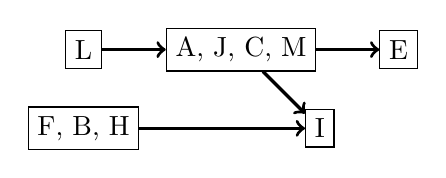
\begin{tikzpicture}
        \node[draw] (E) at (4, 1) {E};
        \node[draw] (L) at (0, 1) {L};
        \node[draw] (AJCM) at (2, 1) {A, J, C, M};
        \node[draw] (I) at (3, 0) {I};
        \node[draw] (FBH) at (0, 0) {F, B, H};

        \draw[->, very thick] (AJCM) -- (E);
        \draw[->, very thick] (L) -- (AJCM);
        \draw[->, very thick] (AJCM) -- (I);
        \draw[->, very thick] (FBH) -- (I);
    \end{tikzpicture}
\end{center}

\section*{Exercise 3}

\begin{enumerate}
    \item Since $a_n: \N \to \Z$ and $a_n$ is strictly decreasing,
          $a_{i} - a_{i+1} > 0 \implies a_{i} - a_{i+1} \geq 1$ since in $\Z$ there are no numbers between two consecutive integers.
          Note that since $a_n$ is strictly decreasing, $a_0$ is the maximum value of $a_n$.
          We conclude that at some $n_0 \leq a_0 + 1$ we have $a_{n_0} < 0$.

    \item Consider the following algorithm:
          \begin{absolutelynopagebreak}
              \begin{minted}{python}
            def find_n0(a):
                # Maximum value of a_n
                N = a(0)

                # Trivial case, a_0 < 0
                if N < 0:
                    return 0
                
                # Trivial case, a_N = 0
                if a(N) = 0:
                    return N + 1

                # We proceed by bisecting the interval [0, N]
                n = N / 2
                while True:
                    # If the current value is negative and 
                    # the previous one is non-negative, we are done
                    if a(n) < 0 and a(n - 1) >= 0:
                        return n

                    # If the current value is non-negative, we need to go right
                    if a(n) >= 0:
                        n = n + (N - n) / 2

                    # If the current value is negative, we need to go left
                    else:
                        n = n / 2
          \end{minted}
          \end{absolutelynopagebreak}

          Note that this algorithm could be implemented also by using recursion, I wrote this version because I came up with this implementation first.

    \item Mathematically, the proof of this is very similar to the proof for Bolzano's Theorem.
          We define 3 sequences by induction:
          \begin{align*}
              j_0 & = 0                      \\
              k_0 & = a_0                    \\
              c_n & = \frac{1}{2}(j_n + k_n) \\
          \end{align*}

          then we check if $a_{c_n}$ is the first negative value (that is $a_{c_n} < 0$ and $a_{c_n - 1} \geq 0$).
          If this is the case, we return $c_n$ and we are done.

          Otherwise we define

          $$
              j_{n+1}=
              \begin{cases}
                  j_n & \text{if } a_{c_n} \geq 0 \\
                  c_n & \text{otherwise}
              \end{cases}
              \quad \text{and} \quad
              k_{n+1}=
              \begin{cases}
                  k_n & \text{if } a_{c_n} < 0 \\
                  c_n & \text{otherwise}
              \end{cases}
          $$

          We have $j_n$ is increasing, $k_n$ is decreasing, and $j_n < b_n$ by construction,
          hence we can be sure that the algorithm will converge to the correct solution.

          The implementation of this algorithm provided above strips away the mathematical details (like creating the sequences $j_n$ and $k_n$)
          and focuses on the practical aspects of the algorithm.

    \item This is a divide-and-conquer algorithm, we can calculate its time complexity as follows:
          $$
              T(N) = T\left(\frac{N}{2}\right) + O(1)
          $$

          where $N = a_0$ is the maximum value of $a_n$.

          Applying the master theorem we have $a = 1$, $b = 2$, and $d = 0$.
          We have $\log_b a = 0 = d$, so the time complexity is $O(\log N)$.
\end{enumerate}

\section*{Exercise 4}

\begin{enumerate}
    \item We prove each implication separately:
          \begin{description}
              \item[$\implies$] If $G$ is bipartite then we color the vertices in $V_1$ with color 1 and the vertices in $V_2$ with color 2.
                  Since there are no edges between vertices of the same set (by definition of bipartite),
                  all the edges go from a vertex of color 1 to a vertex of color 2 and viceversa.
              \item[$\impliedby$] If we can color the vertices of $G$ with 2 colors such that there are no edges between vertices of the same color,
                  then we can define $V_1$ as the set of vertices colored with color 1 and $V_2$ as the set of vertices colored with color 2.
                  Thus $G$ is bipartite with $V_1$ and $V_2$ as the two sets.
          \end{description}
    \item Note that if there are no cycles of odd length it means that all the cycles are of even length.
          We prove each implication separately:
          \begin{description}
              \item[$\implies$] If $G$ is bipartite then for every cycle $C_1, C_2, \ldots, C_n$ in $G$
                  we call $V_1$ the set of vertices that contains $C_1$. Note that $C_2$ must be in $V_2$ since $G$ is bipartite.
                  We repeat the argument for $C_2$ and $C_3$, and so on, and we find that $C_i \in V_1$ if $i$ is odd and $C_i \in V_2$ if $i$ is even.
                  Consider $C_1$ and $C_n$: since $C_1$ has an odd index $C_1 \in V_1$, then $C_n \in V_2$, since they are adjacent, and $n$ must be even.
              \item[$\impliedby$] Perform a DFS on the graph and assign each vertex to either $V_1$ or $V_2$ based on the set of the parent vertex.
                  If the parent vertex is in $V_1$ then the current vertex is in $V_2$ and viceversa.
                  We argument by contradiction: if while exploring $v$ we find an edge $(v, u)$ such that $u$ has already been explored and
                  has been assigned to the same set as $v$, then we have found a cycle. This means that that there exist a path $p$ from $v$ to $u$ that does not include the edge $(v, u)$.
                  We backtrack on $p$ and note that a vertex $p_i$ is in the same set of $v$ if $i$ is even and in the opposite set if $i$ is odd.
                  When we reach $u$ we have that $u$ is in the same set of $v$, hence $u = p_n$ and $n$ is odd.
                  This means that we found a cycle of odd length but this is a contradiction.
          \end{description}

    \item We can use the algorithm described in the previous point in the $\impliedby$ section:
          we perform a DFS on the graph and assign each vertex to either $V_1$ or $V_2$ as described above and immediately halt if we find that an edge $(v, u)$ that connects two vertices in the same set.
          We know that the time complexity of a DFS is $O(|V| + |E|)$, hence the algorithm satisfies the requirements.
\end{enumerate}

\end{document}